\subsection{UC3 - Seleziona file da sincronizzare dal server al client}
\begin{figure}[H]
    \centering
    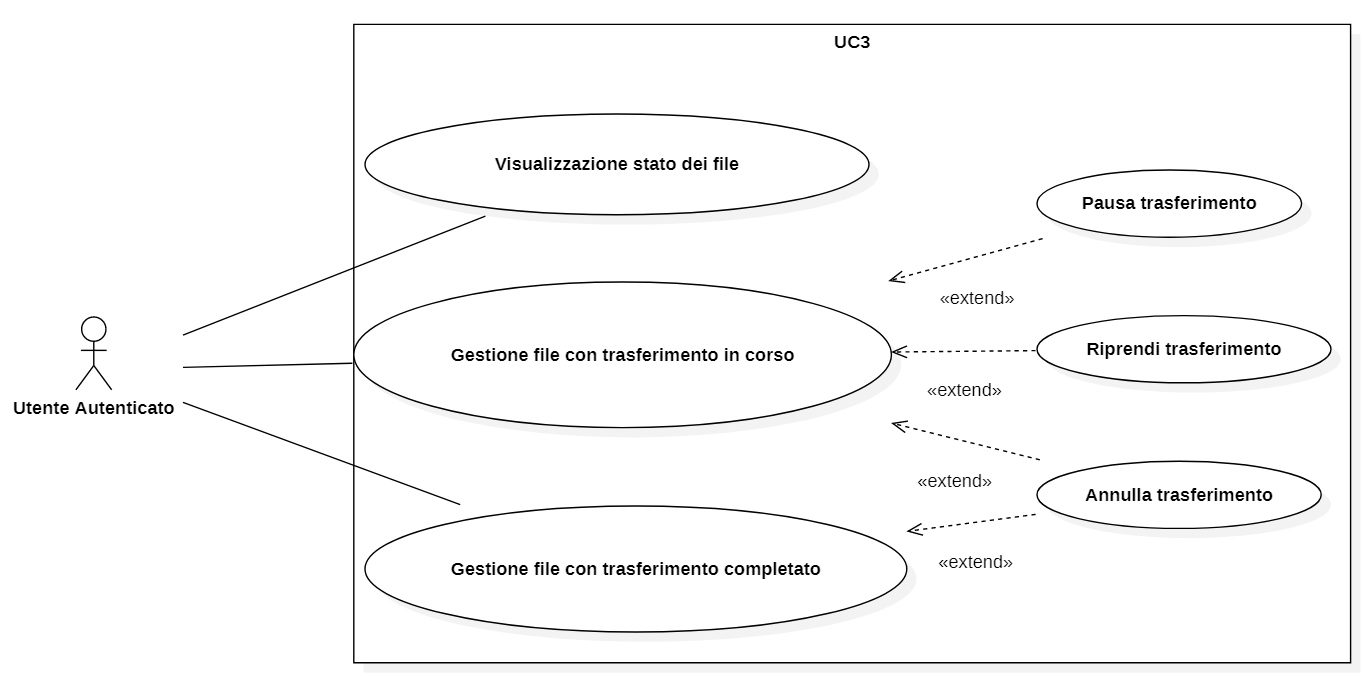
\includegraphics[scale = 0.6]{components/img/UC3.png}
    \caption{UC3 - Seleziona file da sincronizzare dal server al client}
\end{figure}
\subsubsection{UC3.1 - Seleziona file da sincronizzare dal server al client}
\begin{itemize}
\item \textbf{Attore Primario:} Utente autenticato;
\item \textbf{Attore Secondario:} \glo{Zextras Drive};
\item \textbf{Precondizione:} L'utente non ha selezionato nessun file da sincronizzare con il client;
\item \textbf{Postcondizione:} L'utente ha aggiunto dei file che verranno sincronizzati con il client;
\item \textbf{Scenario principale:}
    \begin{enumerate}
    \item L'utente sceglie di aggiungere dei file da sincronizzare con il client;
    \item L'utente aggiunge i file che vuole sincronizzare con il client da una lista presente nell'applicazione;
    \end{enumerate}
\item \textbf{Estensioni:}
    \begin{itemize}
    \item Visualizzazione messaggio di errore di rete (UC7 \S{}\ref{UC7});
    \item Visualizzazione messaggio di errore spazio non disponibile in locale (UC3.2 \S{}\ref{UC3.2}).
    \end{itemize}
\end{itemize}
\subsubsection{UC3.2 - Visualizzazione messaggio di errore spazio non disponibile in locale}
\label{UC3.2}
\begin{itemize}
\item \textbf{Attore Primario:} Utente autenticato;
\item \textbf{Precondizione:} L'utente non ha selezionato nessun file da sincronizzare con il client;
\item \textbf{Postcondizione:} L'utente viene informato che non è stato possibile completare la sincronizzazione;
\item \textbf{Scenario principale:}
    \begin{enumerate}
    \item L'utente ha selezionato i file da sincronizzare;
    \item L'applicazione si connette a \glo{Zextras Drive}, ma fallisce la sincronizzazione per assenza di spazio in locale.
    \end{enumerate}
\end{itemize}